\documentclass[conference]{IEEEtran}

%\usepackage[nocompress]{cite}
\usepackage[english]{babel}
\usepackage{array}
%\usepackage{url}
%\usepackage{amssymb}
%\usepackage{ifthen}
\usepackage{multirow}
\usepackage{csquotes}
\usepackage{fixltx2e}
%\usepackage{enumitem}
%\usepackage{csquotes}
%\usepackage{upquote}
\usepackage{subfigure}
%\setlist{nolistsep}
\usepackage{graphicx}

%common abbreviations
\newcommand{\etal}{{\it et al.}}
\newcommand{\etc}{{\it etc.}}
\newcommand{\ie}{\emph{i.e.}}
\newcommand{\eg}{{\em e.g.}}

%\newboolean{showcomments}
%\setboolean{showcomments}{false}
%
%\ifthenelse{\boolean{showcomments}}
%{ \newcommand{\mynote}[2]{
%    \fbox{\bfseries\sffamily\scriptsize#1}
%    {\small$\blacktriangleright$\textsf{\emph{#2}}$\blacktriangleleft$}}}
%{\newcommand{\mynote}[2]{}}
%
%%Allows to had comments easily with the command \cd{my comment} in the text
%%One command per author (add yours)
%\newcommand{\cd}[1]{\mynote{Corentin}{#1}}
%\newcommand{\ff}[1]{\mynote{Federico}{#1}}
%\newcommand{\todo}[1]{\mynote{TODO}{#1}}

\begin{document}

\title{DC4Cities: Better Usage of the Renewable Energies in Data Centres}

\author{\IEEEauthorblockN{Corentin Dupont}
\IEEEauthorblockA{Create-Net\\
Trento\\
Email: cdupont@create-net.org}
\and
\IEEEauthorblockN{NN 2}
\IEEEauthorblockA{company 2\\
city and code\\
Email: nn@nn.com}
\and
\IEEEauthorblockN{NN 3 etc}
\IEEEauthorblockA{company 3\\
city and code\\
Telephone: xx\\
Fax: xx}}

\maketitle

Energy consumed by data centres in 2010 accounted for between 1.1\% and 1.5\% of the total electricity consumed worldwide~\cite{Koomey2011}, making of data centre energy ma\-nagement an important challenge for researchers.
With the recent adoption of renewable energies to power data centres~\cite{parasol-sigplan2013}, the research community enlarges its vision to associate with purely \emph{quantitative} energy consumption reduction, the notion of \emph{quality} of the energy consumed, \ie\ the capacity to rely as much as possible on sustainable power sources.
Differently from non-renewable energy sources, the availability of renewable energies is very volatile and time dependent: \eg\ solar power is obtainable only during the day, and is subject to variations due to the meteorological conditions.
The goal in this case is to shift the workload of running applications, according to the forecasted availability.

\begin{figure}[ht!]
  \centering
  \subfigure{
     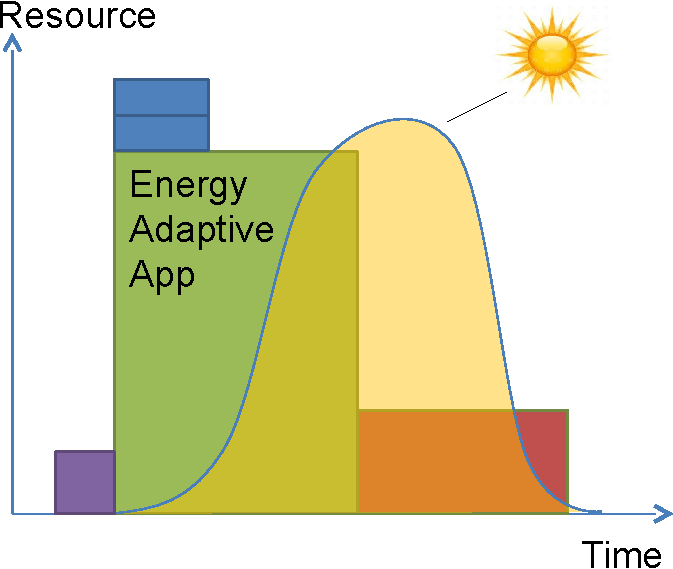
\includegraphics[width=0.42\linewidth]{figs/noadapt}
  }     
  \subfigure{
     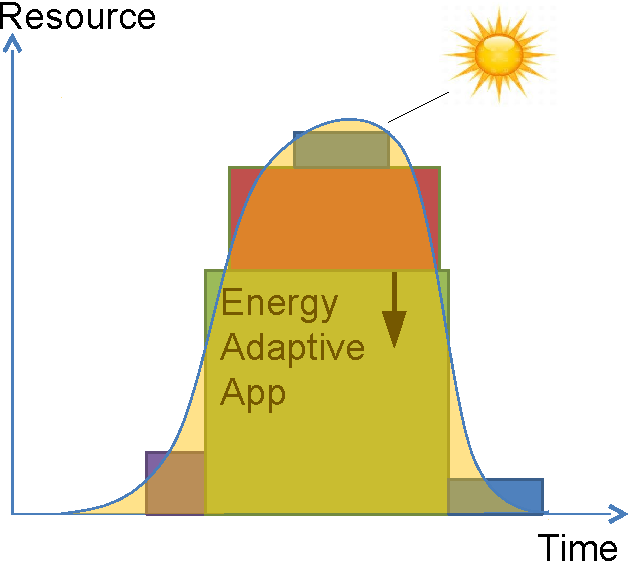
\includegraphics[width=0.40\linewidth]{figs/adapt}
  }     
  \caption{Adapting applications for a better usage of renewable energies}
  \label{fig:adapt}
  \vspace{-1em}
\end{figure}


The scenario that we want to support through our research envisions that an entity external to the data centre, called the Energy Management Authority (EMA), will be able to set high-level energy and power objectives for the data centre.
For example, an objective could be: \enquote{at least 80\% of the data centre energy consumption has to be generated from renewable energy sources}.
To translate these high-level objectives into concrete actions performed in the data centre, the platform developed by DC4Cities will need to be informed about the current and future renewable energy availability.
To this end, the DC4Cities platform will receive forecasts regarding the amount of available power and the energy source mix of its electricity inputs.
These forecasts can be either provided directly by the power suppliers or created by algorithms which use environmental and historical data to predict future renewable energy generation.
Having both workload estimations for the different running applications~\cite{Kansal2008} and the energy forecasts, DC4Cities will be able to assign specific power budgets to the different applications.
The applications, in turn, will have to choose their specific working mode to respect the power budget and the SLAs.

We introduce the concept of Energy Aware Software Controller (EASC).
%initial concepts of DC4Cities, a FP7 project that aims to make data centres more efficient according to the availability of renewable energies.
The EASC implements workload scheduling techniques tightly coupled with energy-adaptive applications that can reconfigure themselves according to power budgets (see Figure~\ref{fig:adapt}).
Each EASC receives a power budget, corresponding to the expected power consumed by the controlled application.
The EASC is then proposing several plans to perform the application's tasks.
Those plans can be controlled using two weighting parameters: the aggressiveness and the eagerness.
The aggressiveness controls the possibility for the application to consume more or less  aggressively the renewable energies.
That is to say, to run at the highest performance level when renewable energies are available, and at the lowest performance when they are not.
The eagerness controls the necessity for an application to perform its tasks early, regardless of the availability of the renewables.
The EASCs are coordinated centrally by the central component of the DC4Cities prototype.
This central component coordinates the EASCs and select the correct plan for each EASC, in order to optimize their combination.

Managing the applications specific workload requires to include in the picture not only the virtual infrastructure layer (IaaS layer) of a data centre, but, as well, the virtual application layer (PaaS layer).
The EASC is able to: (i) manage elasticity and scalability of multi-tier applications according to their energy footprint (\emph{energy-awareness}); (ii) inject mechanisms in the single applications to negotiate energy usage according to energy constraints (\emph{energy-adaptiveness}).

The combination of the above techniques will allow:
\begin{itemize}
  \item optimizing \emph{efficient usage of IT equipment}, making sure the workload is concentrated on the minimal amount of hardware (including shutting down unused ones), while preserving the committed SLAs (including GreenSLAs\footnote{GreenSLAs are SLAs that contain flexibility, green KPIs and collaboration options allowing the data centre to operate in a more energy and emission efficient way.}).
  \item ordering, sequencing, shifting of applications in such a way that IT equipment load, and therefore the data centre power consumption, will \emph{adapt to the energy constraints} coming from the data centre operator and from the energy provider.
  \item cooperating with energy-aware applications to make them reconfigure themselves according to power budgets.
  \item automatic splitting and scheduling of system management activities depending on their energy footprint and their level of criticality.
\end{itemize}

The solutions proposed by DC4Cities has notably been trialled in the data centre of the health agency of the province of Trento, Italy.
Using our prototype, the percentage of renewable energy consumed by the data centre (called REN\%) went from 43.1\% up to 57.9\%. 


\section{Acknowledgments}
The authors would like to thank the EU FP7 project DC4Cities (grant agreement number 609304), and the consortium members.

\bibliographystyle{unsrt}
\bibliography{bibliography/central-bibliography} 

\end{document}

